\documentclass[]{book}

%These tell TeX which packages to use.
\usepackage{array,epsfig}
\usepackage{amsmath}
\usepackage{amsfonts}
\usepackage{amssymb}
\usepackage{amsxtra}
\usepackage{amsthm}
\usepackage{mathrsfs}
\usepackage{color}

%Code Snippits
\usepackage{listings}
\lstset{numbers=left, numberstyle=\tiny, numbersep=5pt}
\lstset{language=Java}

%Tree
\usepackage{tikz}

%Here I define some theorem styles and shortcut commands for symbols I use often
\theoremstyle{definition}
\newtheorem{defn}{Definition}
\newtheorem{thm}{Theorem}
\newtheorem{cor}{Corollary}
\newtheorem*{rmk}{Remark}
\newtheorem{lem}{Lemma}
\newtheorem*{joke}{Joke}
\newtheorem{ex}{Example}
\newtheorem*{soln}{Solution}
\newtheorem{prop}{Proposition}

\newcommand{\lra}{\longrightarrow}
\newcommand{\ra}{\rightarrow}
\newcommand{\surj}{\twoheadrightarrow}
\newcommand{\graph}{\mathrm{graph}}
\newcommand{\bb}[1]{\mathbb{#1}}
\newcommand{\Z}{\bb{Z}}
\newcommand{\Q}{\bb{Q}}
\newcommand{\R}{\bb{R}}
\newcommand{\C}{\bb{C}}
\newcommand{\N}{\bb{N}}
\newcommand{\M}{\mathbf{M}}
\newcommand{\m}{\mathbf{m}}
\newcommand{\MM}{\mathscr{M}}
\newcommand{\HH}{\mathscr{H}}
\newcommand{\Om}{\Omega}
\newcommand{\Ho}{\in\HH(\Om)}
\newcommand{\bd}{\partial}
\newcommand{\del}{\partial}
\newcommand{\bardel}{\overline\partial}
\newcommand{\textdf}[1]{\textbf{\textsf{#1}}\index{#1}}
\newcommand{\img}{\mathrm{img}}
\newcommand{\ip}[2]{\left\langle{#1}
{#2}\right\rangle}
\newcommand{\inter}[1]{\mathrm{int}{#1}}
\newcommand{\exter}[1]{\mathrm{ext}{#1}}
\newcommand{\cl}[1]{\mathrm{cl}{#1}}
\newcommand{\ds}{\displaystyle}
\newcommand{\vol}{\mathrm{vol}}
\newcommand{\cnt}{\mathrm{ct}}
\newcommand{\osc}{\mathrm{osc}}
\newcommand{\LL}{\mathbf{L}}
\newcommand{\UU}{\mathbf{U}}
\newcommand{\support}{\mathrm{support}}
\newcommand{\AND}{\;\wedge\;}
\newcommand{\OR}{\;\vee\;}
\newcommand{\Oset}{\varnothing}
\newcommand{\st}{\ni}
\newcommand{\wh}{\widehat}

%Pagination stuff.
\setlength{\topmargin}{-.3 in}
\setlength{\oddsidemargin}{0in}
\setlength{\evensidemargin}{0in}
\setlength{\textheight}{9.in}
\setlength{\textwidth}{6.5in}
\pagestyle{empty}



\begin{document}


\begin{center}
{\Large Algorithmen und Datenstrukturen \hspace{0.5cm} Sheet 5}
\textbf{Maximilian von Sternberg} %You should put your name here
\end{center}

\vspace{0.2 cm}

\begin{enumerate}
    \item
    \begin{tikzpicture}
        \node[circle,draw](z){15}
          child{
              child {
            node[circle,draw]{7} 
                child{
                    node[circle,draw] {2}
                        child{
                            node[circle,draw] {1}
                            } 
                        child{
                            node[circle,draw] {6}
                    } 
                    } 
                child{
                    node[circle,draw] {8}
                } 
              }
              child[missing]
          }
          child{
              child[missing] {}
              child{
            node[circle,draw]{18} 
                child{
                child{
                    node[circle,draw] {16}
                    child{
                        node[circle,draw] {13}
                        } 
                    child{
                        node[circle,draw] {17}
                } 
                    } child[missing]}
                child{
                    node[circle,draw] {21}                        
                    child{
                        node[circle,draw] {20}
                        } 
                    child{
                        node[circle,draw] {22}
                } 
                } }
            };
        \end{tikzpicture}
        \begin{description}
            \item addRoot(15)
            \item addLeft(15, 7)
            \item addRight(15, 18)
            \item addLeft(7, 2)
            \item addRight(7, 8)
            \item addLeft(2, 1)
            \item addRigt(2, 6)
            \item addLeft(18, 16)
            \item addRight(18, 21)
            \item addLeft(16, 13)
            \item addRight(16, 17)
            \item addLeft(21, 20)
            \item addRight(21, 22)
        \end{description}
    \item \begin{enumerate}
        \item Wenn alle Blatt-Knoten diesselbe Tiefe besitzen
        \item \begin{align*}
            H  = \log_2(N + 1) - 1 \quad &|+ 1\\ 
            H + 1 = \log_2(N + 1)  \quad &|2^{()}\\ 
            2^{H + 1}  = N + 1 \quad &|-1\\ 
            2^{H + 1} - 1  = N &\qed
        \end{align*}
        \item \begin{align*}
            n_E & \le 2^h \quad |\log_2\\ 
            log_2 n_E & \le h \qed
        \end{align*}
    \end{enumerate}
    \item \lstinputlisting[frame=single,label=beispielcode,caption=Ein Beispiel]{BreadthFirstIterator.java}

    
\end{enumerate}

\end{document}
